\chapter[Considerações finais]{Considerações finais}

Como foi apresentado ao longo deste trabalho, a comunidade de robótica busca solucionar o problema de SLAM utilizando diversas técnicas e estratégias. Entretanto, boa parte da comunidade concorda na utilização de algumas estratégias, como o processamento remoto, apresentado na tabela \ref{tab:resultadosRevisao}. Visto isso, este trabalho buscará seguir as estratégias mais utilizadas e mais úteis para o contexto de pesquisa, como a utilização da arquitetura de processamento remoto e filtros probabilísticos.

A escolha do filtro probabilístico a ser utilizado depende de etapas de provas de conceito que serão realizadas durante as primeiras sprints de desenvolvimento do TCC\_2. A escolha será entre a utilização do filtro de Kalman ou do filtro de Partículas, ambos detalhados ao decorrer deste trabalho.

A escolha da linguagem de programação utilizada, Java, se dá pela necessidade de integração com o \textit{framework} Traveller, além da facilidade e apoio disponíveis com a utilização da ferramenta \textit{Lejos}. Os conhecimentos obtidos durante a realização da prova de conceito comprovam que a escolha da utilização da linguagem Java possibilita maior suporte técnico, como materiais e conteúdos na \textit{web}, o que facilita o desenvolvimento do trabalho como um todo.

Ao longo do TCC\_1, o foco do trabalho foi levantar técnicas e estratégias existentes para resolução do problema de SLAM, assim como identificar conceitos e informações referentes à auto-localização na robótica e robótica educacional. Desse modo, levando em consideração os objetivos específicos, a Figura \ref{img:porcentagemFinal} apresenta o \textit{status} do trabalho.

\begin{figure}[H]
	\centering
	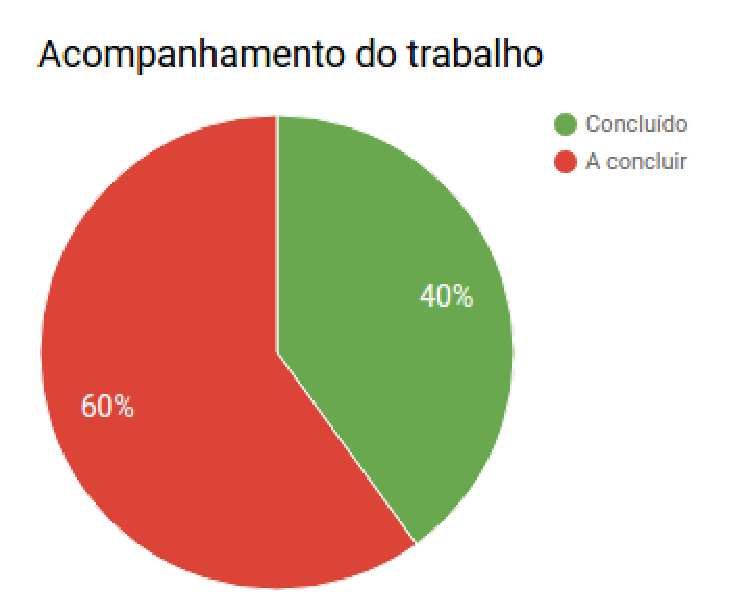
\includegraphics[scale=0.6]{figuras/porcentagem.eps}
	\label{img:porcentagemFinal}
	\caption[Trabalho desenvolvido]{Trabalho desenvolvido}
\end{figure}

Os objetivos específicos foram registrados como:

\begin{itemize}
	\item Identificar uma solução para o problema de SLAM em um contexto simplificado;
	\item Propor adaptação para o contexto de robôs simples, na Robótica Educacional;
	\item Implementar adaptação.
\end{itemize}

Desse modo, durante a primeira etapa da pesquisa (TCC\_1), foi possível identificar uma solução para o problema de SLAM em um contexto simpificado, a partir da análise do resultado da revisão sistemática. A proposta de adaptação foi realizada em parte, já que já foi definida a utilização da arquitetura de processamento remoto e a seleção de dois filtros probabiĺísticos que serão utilizados na adaptação. Ou seja, aproximadamente 40\% do trabalho foi concluído, o que está dentro do previsto, pois o período destinado para a realização da segunda etapa (TCC\_2) é maior, já que é referente a uma disciplina de seis créditos, diferentemente da primeira etapa.